\documentclass{ximera}

\title{Gradient Descent Basics}
\author{Zack Reed}

\begin{document}
\begin{abstract}
In this activity we gain some initial intuitions behind gradient descent, a fundamental algorithm for multivariable optimization.
\end{abstract}
\maketitle

\section*{Introduction: Why Gradients?}


\begin{remark}

We touched on this in the previous module, but it becomes very important for optimization: The gradient vector points in the direction of steepest \textbf{increase} of the function.

This means that to \textbf{increase} the function value most rapidly, you should move in the direction of the gradient vector. Conversely, to \textbf{decrease} the function value most rapidly (i.e., to minimize), you should move in the \textbf{opposite} direction of the gradient vector.

\end{remark}

The following video provides a brief intuition for why the gradient points in the direction of steepest increase.

\begin{center}
    \youtube{TEB2z7ZlRAw?si=BbbmRIUfRkqNQ3dT}
\end{center}

\begin{problem}
Consider the following function: $f(x,y) = x^2 + y^2$.

Suppose we are at the point $(1,1)$. In what direction should we move to most dramatically \textbf{decrease} the function value?

\begin{multipleChoice}
    \choice{Towards the origin $(0,0)$}
    \choice{In the direction of the vector $\langle -2, -1 \rangle$}
    \choice{In the direction of the vector $\langle 2, 2 \rangle$}
    \choice[correct]{In the direction of the vector $\langle -2, -2 \rangle$}
    \choice{Along the $x$-axis}
    \choice{Along the $y$-axis}
    \choice{In the direction of the vector $\langle 1, 2 \rangle$}
\end{multipleChoice}
\end{problem}

This is the first key insight for optimization: To minimize a function, we should move in the direction of the \textbf{negative} gradient. The question that remains is \textbf{how far} to move in that direction. We'll answer that question next.

\subsection*{The Gradient Descent Algorithm}

When you imagine gradient descent, you want to imagine rolling a ball down a hill. If the bottom of the hill is a small bowl, the ball will hit the bowl, maybe roll around a bit, and eventually settle at the bottom.

This intuition is conveyed in the following animation. Note that arrows point the direction in which the ball should move to roll downhill. The arrow represents the gradients we will calculate in higher dimensional settings.

\begin{center}
    \youtube{HZr6lsyinaE}
\end{center}

Here's how gradient descent works:

\begin{enumerate}
    \item Start at an initial point $(x_0, y_0)$
    \item Compute the gradient $\nabla f(x_0, y_0)$
    \item Take a small step in the \textbf{opposite} direction: 
    $$\begin{pmatrix} x_1 \\ y_1 \end{pmatrix} = \begin{pmatrix} x_0 \\ y_0 \end{pmatrix} - \alpha \nabla f(x_0, y_0)$$
    where $\alpha$ is step size. Often, $\alpha$ is called the \textbf{learning rate}.
    \item Repeat until the gradient is nearly zero
\end{enumerate}

\begin{problem}
Let's manually perform one step of gradient descent on $f(x,y) = x^2 + y^2$.

Starting at $(x_0, y_0) = (4, 3)$ with learning rate $\alpha = 0.1$:

The gradient at $(4,3)$ is $\nabla f(4,3) = \langle \answer{8}, \answer{6} \rangle$

We move opposite to the gradient:

$$\begin{pmatrix} x_1 \\ y_1 \end{pmatrix} = \begin{pmatrix} 4 \\ 3 \end{pmatrix} - 0.1 \begin{pmatrix} 8 \\ 6 \end{pmatrix}$$

So $x_1 = \answer{3.2}$ and $y_1 = \answer{2.4}$

The function value decreased from $f(4,3) = \answer{25}$ to $f(3.2, 2.4) = \answer[tolerance=0.1]{16}$.

%a visual of the step
\begin{center}
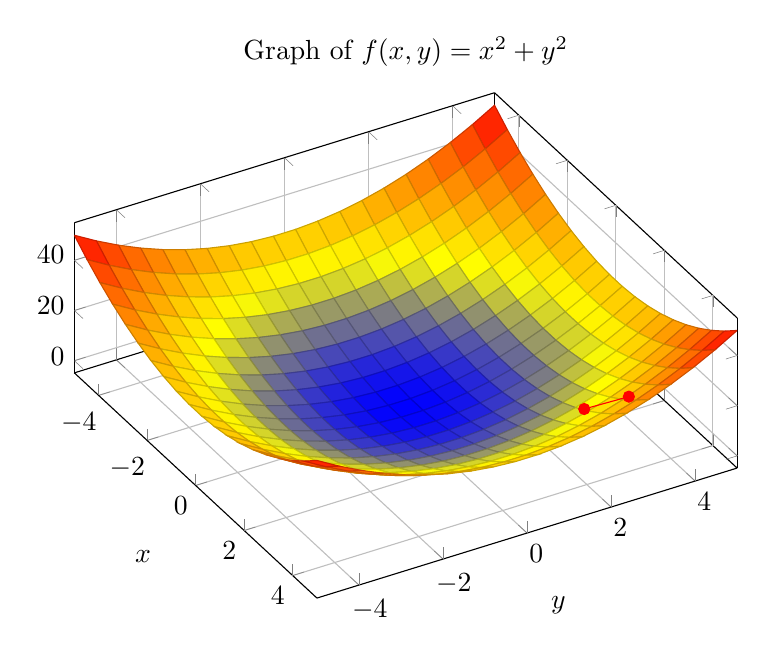
\begin{tikzpicture}
    \begin{axis}[
        domain=-5:5,
        samples=50,
        xlabel = $x$,
        ylabel = {$y$},
        title = {Graph of $f(x,y) = x^2 + y^2$},
        width=10cm,
        height=8cm,
        grid=major,
        view={60}{60},
    ]
    \addplot3[surf,domain=-5:5,y domain=-5:5,samples=20] {x ^2 + y ^2};
    \addplot3[mark=*, color=red] coordinates {(4,3,25) (3.2,2.4,16)};
    \end{axis}
\end{tikzpicture}
\end{center}

\begin{feedback}
    We moved closer to the minimum at $(0,0)$! Repeating this process many times converges to the minimum.
\end{feedback}
\end{problem}

The following animation shows this playing out on a bumpy surface. Imagine dropping many balls all over the surface, note that the balls will settle not in a single minimum point, but in the nearest minimum point to the ball's starting location.

\begin{center}
    \youtube{82PyiYVCsGk}
\end{center}

In the next activity, we'll learn more about why the learning rate is important and how to choose it wisely.


\end{document}
